\documentclass[12pt]{article}
\usepackage{setspace, graphicx, fullpage, amssymb, amsmath, epsfig, natbib, array, multirow, hyperref}
\usepackage{amsfonts, bm} 
\usepackage{dcolumn}
\usepackage{subfigure, float} 
\usepackage[margin=1in]{geometry} 
\usepackage{verbatim}
\usepackage{url}
\usepackage{enumerate}
\usepackage{morefloats}
\newcolumntype{d}[1]{D{.}{.}{#1}} 



\begin{document}
	
\begin{center}
	\Large 22 March 2017
\end{center}

\section{Overview}

At our previous meeting we decided to do the following:
\begin{itemize}
	\item Rewrite sections of the first draft in order to better describe what the contribution of Minozzi \& Volden (2013) was in order to frame our replication, enter more fully into the conversation on elections and induced preferences, and discuss the fact that on non-party calls extremists walk away from the party just like moderates.
	
	\item Develop coefficient plots to replace the tables for the diff-in-diff/coherence design
	
	\item Write appendices which cover differences from the House sorting model and the reelection matching
	
	\item Write a single R script which creates all the tables and figures we are considering using in this paper
	
	\item Create a separate \LaTeX document which contains tables and figures we would want to include in a second paper focused on increases in party calls over Congresses 93-112
\end{itemize}



\pagebreak

\section{Paper, Draft 2}

\subsection{Introduction}

Minozzi \& Volden (2013) showed that a significant factor in achieving party unity comes not from pressuring moderates but calling on members to coalesce out of shared interest. More extreme members in the party were hypothesized and shown to be the most responsive to the ``party call'' because they gain the most both from the status of the party and their status as a partisan in most cases. Extreme members who already have strong preferences on an issue would be unlikely to see this preference change, but those whose preferences are weaker will see the call as a clear reason to align for the good of the party.

This paper works to replicate these findings and extend them into Congresses 110-112 in the House as well as into the Senate. This allows us to test the responsive extremists hypothesis in times that the party is thought to be getting more extreme in the House. We can also test if it holds when applied to the Senate in order to see if it is a quirk of the House or a trait of Congressional behavior generally. We hypothesize that these relationships will be largely the same. Further, the inclusion of the Senate allows us to consider the influence of proximity to reelection in choosing whether to heed the call of the party.

Mayhew (1974) shows that reelection is chief among the desires of members of Congress. Canes-Wrone, Brady \& Cogan (2002) shows that members who stray to far from the preferences of their district are less likely to be reelected. While this would initially seem to imply that members would act according to the preferences of their district above those of their party, we know from Lee (2009) that the name brands of parties confer advantages on members and that members are thus willing to take actions and positions that are either beneficial to their own party relative to the opposition. and Carson, Koger, Lebo \& Young (2010) that following the party line too closely can in itself be electorally costly to an individual member. Levitt (1996) finds that proximity to reelection induces Senators to more strongly take their constituents' preferences into account. If members only respond to party calls when they do not have strong preferences against the party and proximity to reelection increases the attention they pay to their constituents' preferences, we should expect that members will be less responsive to party calls in Congresses which they are up for reelection.

\subsection{Replication with Extension}

In this section we show that the results from Minozzi \& Volden (2013) hold when analysis is extended into later Congresses and the Senate. We draw on Congressional roll call data for Congresses 93-112 for both chambers in order to view the behavior of members. As in Minozzi \& Volden (2013), we iteratively sort votes based on the the predictive power of party in vote decision taken alongside party free ideology. We dub those votes which are significantly predicted by party as party calls and those which are not as noncalls. The set of noncalls from one iteration is used as the votes for calculating party free ideology in the next. A more thorough overview of the original algorithm and the changes we've made to it are detailed in an appendix.

We make a number of important findings. First, the relationship between extremism and vote choice is not random with both extremists and moderates of each party likely to vote against the party on non party call votes, but on party call votes the extremists snap intoline with the party. The relationship we find between ideological extremism and party call responsiveness, shown in figures 1 and 2 demonstrates this as a percent. The nonlinearity between party call response rate and ideological extremism appears to arise from the fact that there is a maximum rate of 100\%.

\begin{figure}[H]
	\centering
	\caption{House Rate of Voting With Party by Vote Type}
	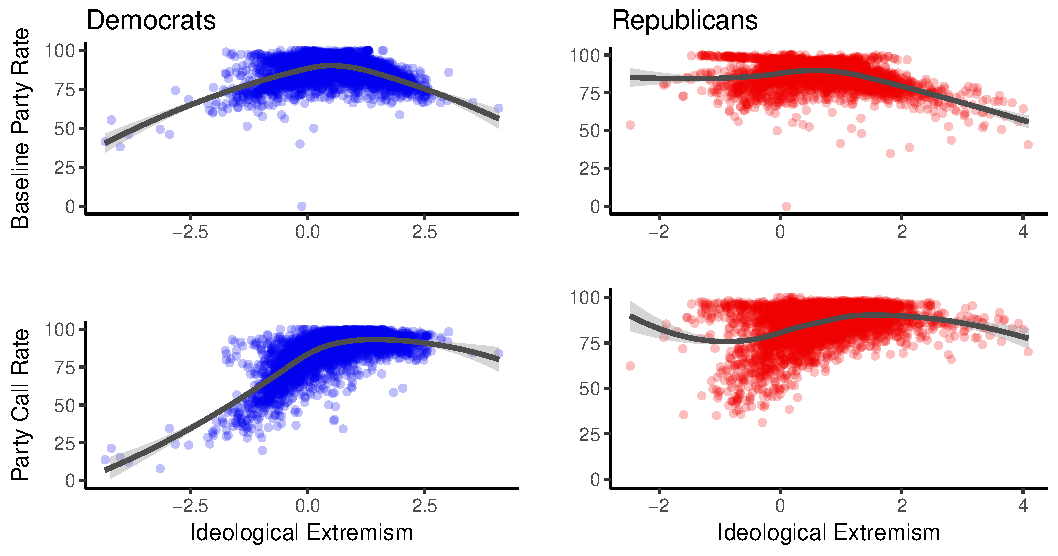
\includegraphics[width = \textwidth]{C:/Users/Ethan/Documents/GitHub/partycalls/plots/house_responsiveness_plot.pdf}
\end{figure}

\begin{figure}[H]
	\centering
	\caption{Senate Rate of Voting With Party by Vote Type}
	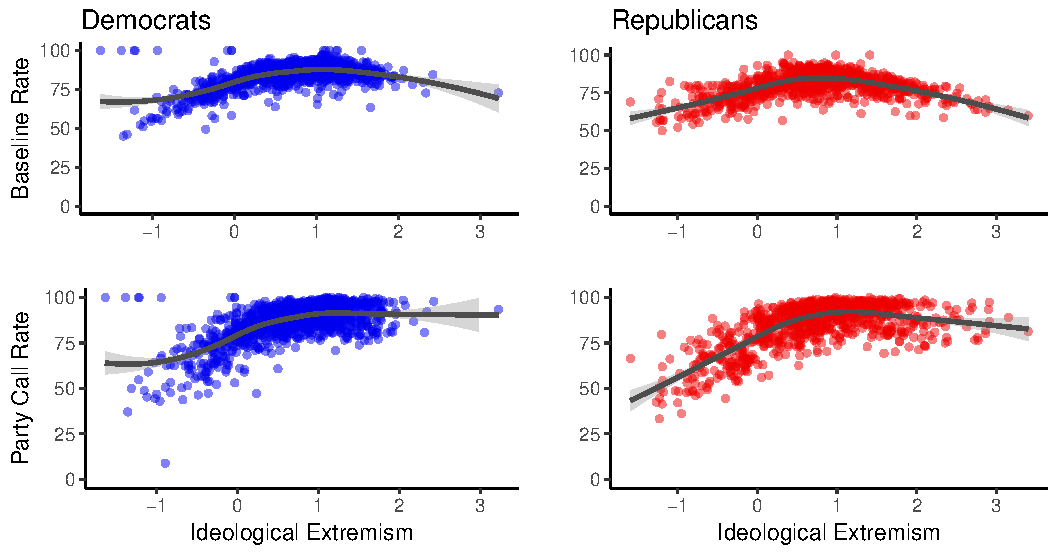
\includegraphics[width = \textwidth]{C:/Users/Ethan/Documents/GitHub/partycalls/plots/senate_responsiveness_plot.pdf}
\end{figure}

We also note that the number of party call votes in both chambers of Congress during the period of analysis are on an upward trend. We believe this trend merits further investigation, but initially take it to echo arguments such as those of Lee (2009), Theriault (2013), and Smith (2014) that Congressional partisan conflict has been on the rise. 

\begin{figure}[H]
	\centering
	\caption{Party Calls as a Percentage of Votes, Congresses 93-112}
	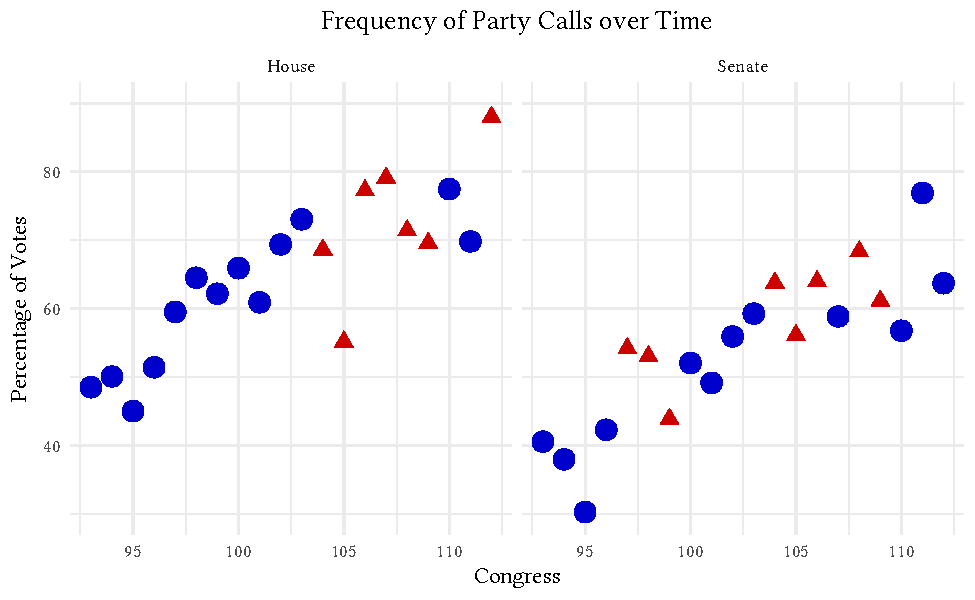
\includegraphics[width = \textwidth]{C:/Users/Ethan/Documents/GitHub/partycalls/plots/party_call_percent_both.pdf}
\end{figure}

Pooled regressions with members divided by party and majority status broadly show similar relationships both between chambers in the current analysis as well as with those presented in Minozzi \& Volden (2013). Though they differ in strength between parties, ideological extremism and rate of voting with majority of non party call votes both carry substantive predictive power in determining responsiveness by to party calls. 

Unsurprisingly, in both chambers we also find that southern Democrats are less responsive to the party than are other Democrats. We also note that the power committee variable we constructed for the Senate (based on membership in a top 4 committee) carries little predictive power, either in terms of substantive power or statistical significance. This is unsurprising since this is a variable we included less because we believed it had meaning to Senators and more for model comparability. We also note that in both chambers increased same party presidential vote share within one's constituency makes Democrats more likely to respond to a party call but reduces the chances of a Republican doing so.

\begin{table}[H]
	\begin{center}
		\caption{House Responsiveness to Party Calls, Pooled Regressions}
		%\footnotesize
		\begin{tabular}{l c c c c }
			\hline
			& Democrats & Republicans & Majority & Minority \\
			\hline
			ideological\_extremism & $8.34^{***}$  & $5.84^{***}$  & $6.65^{***}$  & $8.73^{***}$  \\
			& $(0.17)$      & $(0.21)$      & $(0.16)$      & $(0.20)$      \\
			pfrate100              & $0.64^{***}$  & $0.41^{***}$  & $0.52^{***}$  & $0.64^{***}$  \\
			& $(0.02)$      & $(0.02)$      & $(0.01)$      & $(0.02)$      \\
			votepct                & $-0.04^{***}$ & $-0.00$       & $-0.09^{***}$ & $-0.07^{***}$ \\
			& $(0.01)$      & $(0.01)$      & $(0.01)$      & $(0.01)$      \\
			pres\_votepct          & $0.09^{***}$  & $-0.09^{***}$ & $0.20^{***}$  & $0.16^{***}$  \\
			& $(0.01)$      & $(0.02)$      & $(0.01)$      & $(0.02)$      \\
			south                  & $-2.43^{***}$ & $3.63^{***}$  & $-1.64^{***}$ & $-0.38$       \\
			& $(0.28)$      & $(0.34)$      & $(0.25)$      & $(0.31)$      \\
			female                 & $0.53$        & $-0.08$       & $-0.14$       & $2.12^{***}$  \\
			& $(0.35)$      & $(0.57)$      & $(0.40)$      & $(0.44)$      \\
			afam                   & $-0.52$       & $5.01$        & $-3.04^{***}$ & $3.25^{***}$  \\
			& $(0.44)$      & $(2.97)$      & $(0.53)$      & $(0.61)$      \\
			latino                 & $1.73^{***}$  & $2.41^{*}$    & $2.82^{***}$  & $3.02^{***}$  \\
			& $(0.51)$      & $(1.15)$      & $(0.63)$      & $(0.70)$      \\
			seniority              & $0.05$        & $-0.33^{***}$ & $0.01$        & $0.01$        \\
			& $(0.03)$      & $(0.05)$      & $(0.03)$      & $(0.04)$      \\
			freshman               & $-0.07$       & $1.00^{*}$    & $0.24$        & $-0.41$       \\
			& $(0.36)$      & $(0.46)$      & $(0.35)$      & $(0.45)$      \\
			bestgrosswart          & $-0.04^{*}$   & $-0.24^{***}$ & $-0.18^{***}$ & $-0.16^{***}$ \\
			& $(0.02)$      & $(0.03)$      & $(0.02)$      & $(0.02)$      \\
			leader                 & $1.96^{**}$   & $2.80^{***}$  & $2.61^{***}$  & $1.78^{**}$   \\
			& $(0.60)$      & $(0.76)$      & $(0.65)$      & $(0.65)$      \\
			power                  & $1.82^{***}$  & $2.95^{***}$  & $3.02^{***}$  & $1.06^{**}$   \\
			& $(0.28)$      & $(0.37)$      & $(0.27)$      & $(0.36)$      \\
			chair                  & $2.49^{***}$  & $9.85^{***}$  & $1.86^{***}$  &               \\
			& $(0.50)$      & $(0.80)$      & $(0.44)$      &               \\
			(Intercept)            & $24.00^{***}$ & $53.04^{***}$ & $36.45^{***}$ & $17.69^{***}$ \\
			& $(1.58)$      & $(2.21)$      & $(1.49)$      & $(2.05)$      \\
			\hline
			R$^2$                  & 0.63          & 0.30          & 0.57          & 0.48          \\
			Adj. R$^2$             & 0.63          & 0.30          & 0.57          & 0.48          \\
			Num. obs.              & 4746          & 3798          & 4898          & 3646          \\
			RMSE                   & 7.36          & 8.87          & 7.54          & 8.02          \\
			\hline
			\multicolumn{5}{l}{\scriptsize{$^{***}p<0.001$, $^{**}p<0.01$, $^*p<0.05$}}
		\end{tabular}
	\end{center}
\end{table}

\begin{table}[H]
	\begin{center}
		\caption{Senate Responsiveness to Party Calls, Pooled Regressions}
		%\footnotesize
		\begin{tabular}{l c c c c }
			\hline
			& Democrats & Republicans & Majority & Minority \\
			\hline
			ideological\_extremism & $3.14^{***}$ & $7.79^{***}$  & $4.82^{***}$  & $7.98^{***}$ \\
			& $(0.41)$     & $(0.36)$      & $(0.31)$      & $(0.39)$     \\
			pfrate100              & $0.76^{***}$ & $0.74^{***}$  & $0.70^{***}$  & $0.72^{***}$ \\
			& $(0.03)$     & $(0.03)$      & $(0.03)$      & $(0.03)$     \\
			up\_for\_reelection    & $-0.63$      & $-1.44^{**}$  & $-0.94^{*}$   & $-0.97$      \\
			& $(0.43)$     & $(0.54)$      & $(0.41)$      & $(0.58)$     \\
			vote\_share            & $-0.05^{*}$  & $0.15^{***}$  & $-0.01$       & $0.07^{*}$   \\
			& $(0.02)$     & $(0.03)$      & $(0.02)$      & $(0.03)$     \\
			pres\_vote\_share      & $0.23^{***}$ & $-0.13^{***}$ & $0.18^{***}$  & $0.02$       \\
			& $(0.02)$     & $(0.03)$      & $(0.02)$      & $(0.03)$     \\
			south                  & $-1.69^{**}$ & $0.87$        & $-0.09$       & $1.18^{*}$   \\
			& $(0.56)$     & $(0.58)$      & $(0.42)$      & $(0.59)$     \\
			female                 & $1.69^{*}$   & $0.45$        & $0.73$        & $3.51^{**}$  \\
			& $(0.73)$     & $(1.13)$      & $(0.72)$      & $(1.07)$     \\
			afam                   & $-1.16$      & $-10.79^{*}$  & $1.32$        & $-5.19$      \\
			& $(2.79)$     & $(4.28)$      & $(4.21)$      & $(3.18)$     \\
			latino                 & $1.81$       & $7.26^{**}$   & $4.73^{*}$    & $6.06$       \\
			& $(2.20)$     & $(2.78)$      & $(1.89)$      & $(3.47)$     \\
			seniority              & $0.04$       & $-0.02$       & $0.05$        & $0.12$       \\
			& $(0.05)$     & $(0.07)$      & $(0.06)$      & $(0.07)$     \\
			freshman               & $0.77$       & $0.36$        & $0.48$        & $0.91$       \\
			& $(0.71)$     & $(0.84)$      & $(0.62)$      & $(1.00)$     \\
			retiree                & $1.60$       & $2.29^{*}$    & $1.73^{*}$    & $2.40^{*}$   \\
			& $(0.90)$     & $(1.00)$      & $(0.85)$      & $(1.07)$     \\
			best\_committee        & $0.24$       & $0.01$        & $0.03$        & $0.37^{*}$   \\
			& $(0.12)$     & $(0.15)$      & $(0.12)$      & $(0.17)$     \\
			leader                 & $2.22^{**}$  & $0.91$        & $1.51^{*}$    & $1.84^{*}$   \\
			& $(0.71)$     & $(0.78)$      & $(0.64)$      & $(0.87)$     \\
			power\_committee       & $-0.85$      & $-0.32$       & $-0.07$       & $-1.45$      \\
			& $(0.77)$     & $(0.92)$      & $(0.71)$      & $(1.02)$     \\
			chair                  & $0.85$       & $3.63^{***}$  & $0.21$        & $-10.87$     \\
			& $(0.54)$     & $(0.70)$      & $(0.51)$      & $(7.70)$     \\
			(Intercept)            & $9.45^{**}$  & $18.18^{***}$ & $16.69^{***}$ & $8.74^{*}$   \\
			& $(2.91)$     & $(3.49)$      & $(2.63)$      & $(3.83)$     \\
			\hline
			R$^2$                  & 0.69         & 0.64          & 0.68          & 0.62         \\
			Adj. R$^2$             & 0.68         & 0.64          & 0.67          & 0.61         \\
			Num. obs.              & 1042         & 951           & 1100          & 893          \\
			RMSE                   & 6.12         & 7.25          & 5.91          & 7.67         \\
			\hline
			\multicolumn{5}{l}{\scriptsize{$^{***}p<0.001$, $^{**}p<0.01$, $^*p<0.05$}}
		\end{tabular}
	\end{center}
\end{table}

In Table 2, we see some evidence of differences between members up for reelection and others. Though it fails to meet traditional significance threshold for Democrats, across all subgroups this coefficient is negative. 

\subsection{Reelection in the Senate}

In this section we estimate models which account for variation within members, using same-state Senator pairs in Congresses which one of them is up for reelection. Such pairings have the advantage of answering to the same constituents. In order to estimate the effect of reelection on member responsiveness we use generalizations of the difference in differences design which compare member responsiveness to the party on party calls, the baseline rate of voting with the party, and the difference between these two quantities along with bootstrapped 95\% confidence intervals. For each of these a placebo test with randomly assigned treatment is also shown. These tests is further detailed in an appendix.

\begin{figure}[H]
	\centering
	\caption{Senate Rate of Voting With Party by Vote Type}
	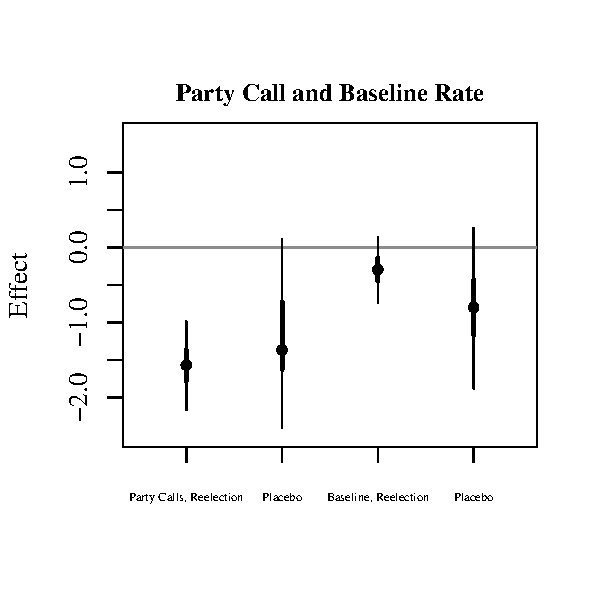
\includegraphics[width = 10cm]{C:/Users/Ethan/Documents/GitHub/partycalls/plots/senate-diff-in-diff-coeff-separate.pdf}
\end{figure}

\begin{figure}[H]
	\centering
	\caption{Senate Rate of Voting With Party by Vote Type}
	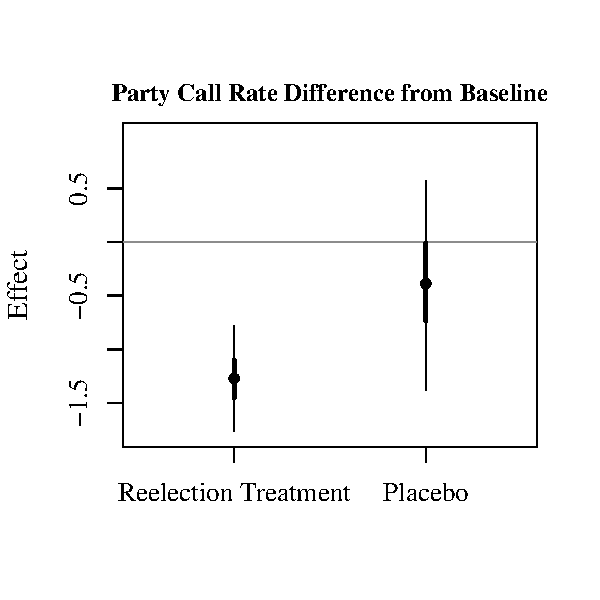
\includegraphics[width = 10cm]{C:/Users/Ethan/Documents/GitHub/partycalls/plots/senate-diff-in-diff-coeff.pdf}
\end{figure}

These show clearly that member responsiveness to party calls declines by approximately 1.5\%. Since the average number of party calls in a Congress during the time we analyze is approximately 365, this means that a Senate party can generally expect to count on members up for reelection for a little over 5 votes against the party on party call votes. Member voting behavior on other votes is negatively signed but fails to meet traditional thresholds of statistical significance and member behavior on party calls when compared to their baseline rate of voting with the party is comparable to that of the changes present in their party call rate generally.

\subsection{Conclusion}

In this paper, we show that members respond to party calls in the Senate as they do in the House using similar analysis to Minozzi \& Volden (2013). Further, in the Senate we are able to consider the role that proximity to reelection has in responsiveness to the party in Congress. This allows us to extend analyses which have focused on behavior in Congress in more general manners and focus in on those areas where differences are most present. Across multiple statistical tests we find that in Congresses which a member is up for reelection there is a lowered responsiveness to the party, especially amongst Republicans.

\pagebreak

\section{Appendices}

\subsection{Appendix A: Detailing the New Sorting Algorithm}

As in Minozzi \& Volden (2013) we develop an algorithm to sort votes based on the degree to which vote choice can be significantly predicted by party when vote choice is modeled by party and ideology. This algorithm works iteratively, with member ideology in one iteration calculated on the votes which were not party calls in the previous iteration, with the ideology for the first iteration being set as votes which have more than 65\% or less than 35\% of members voting on a bill on the same side. The algorithm must run 15 iterations per Congress as a burn-in period. Once this period has concluded the algorithm continues either until the number of votes switched has hit a minimum and begun to climb or until there are fewer than 5 votes which switch between iterations. Once these conditions are met, it continues for 15 additional iterations, the last 5 of which are used to identify party calls and non calls. Any votes which switched between party calls and non party calls during the final five iterations are dropped from our analyses.

We find that the results produced by the algorithm largely do not involve a tradeoff of party and ideology explaining votes, but instead typically have both explaining effects in the same direction. We have made some changes to this algorithm, which are detailed below.

% latex table generated in R 3.3.2 by xtable 1.8-2 package
% Thu Feb 23 17:39:42 2017
\begin{table}[H]
	\centering
	\caption{House Sorting Algorithm Coefficient Signs}
	\begin{tabular}{rrr}
		\hline
		& ($-$) Ideal & (+) Ideal \\ 
		\hline
		(-) Party & 0.38 & 0.15 \\ 
		(+) Party & 0.17 & 0.30 \\ 
		\hline
	\end{tabular}
\end{table}

% latex table generated in R 3.3.2 by xtable 1.8-2 package
% Thu Feb 23 17:23:31 2017
\begin{table}[H]
	\centering
	\caption{Senate Sorting Algorithm Coefficient Signs}
	\begin{tabular}{rrr}
		\hline
		& ($-$) Ideal & (+) Ideal \\ 
		\hline
		($-$) Party & 0.33 & 0.16 \\ 
		(+) Party & 0.23 & 0.28 \\ 
		\hline
	\end{tabular}
\end{table}

One of the key changes was the use of the \verb|emIRT()| R function as described in Imai, Lo \& Olmsted (2016) in order to obtain members' party free ideology. This function was developed by Imai and co-authors in order to produce estimates analagous to those of the \verb|ideal()| function developed by Clinton, Jackman \& Rivers (2004), which was used by Minozzi \& Volden (2013). A key advantage of this new function for estimation of member ideology is that it produces results with greatly reduced computation.

We found that the lowered number of both members and bills in the Senate required a few changes to the vote sorting method. First, since p-values will necessarily be lower with fewer observations, we had to change the p-value threshold for party significance to 0.05 (from 0.01). Next, since the ideal point algorithm uses a logistic regression problems arose in vote sorting when we also tried to use a logistic regression in the Senate and changed to using a linear model. Neither change leads the sorting in the House to change drastically and we find that the sorting of votes based on whether they are close or lopsided mirrors that found in Minozzi \& Volden (2013) very closely.

% latex table generated in R 3.3.2 by xtable 1.8-2 package
% Mon Mar 20 13:02:44 2017
\begin{table}[H]
	\centering
	\caption{House Vote Coding for Close and Lopsided Votes} 
	\begin{tabular}{lrr}
		\hline
		& Party Call & Noncall \\ 
		\hline
		Lopsided & 4245 & 6123 \\ 
		Close & 9308 & 1090 \\ 
		\hline
	\end{tabular}
\end{table}

% latex table generated in R 3.3.2 by xtable 1.8-2 package
% Mon Mar 20 13:04:18 2017
\begin{table}[H]
	\centering
	\caption{Senate Vote Coding for Close and Lopsided Votes} 
	\begin{tabular}{lrr}
		\hline
		& Party Call & Noncall \\ 
		\hline
		Lopsided & 2063 & 4876 \\ 
		Close & 5233 & 1851 \\ 
		\hline
	\end{tabular}
\end{table}













\subsection{Appendix B: Methodology for Senate Reelection Section}

In order to better test the role of reelection we use same-state senators as a natural pairing. We view this as an ideal pairing since they answer to the same possible set of voters and therefore should have similar preferences induced by proximity to reelection. The tests we performed on these pairs were generalizations of the difference in differences design in which the member not up for reelection had their response rate subtracted from that of the member who was up for reelection for the first figure in the paper and for the second members had the difference between their party call response rate and baseline rate of voting with the party subtracted from that of the other Senator from their state under the same conditions. 

Here we show the effects in tables, along with breakdowns by seat pair type. We additionally show the results of a model with fixed effects by member and Congress. This produces substantively similar effects to those reported in the main paper on the effects of being up for reelection and changes in ideological extremism. This is presented as a robustness check for the results we present in the paper.

% latex table generated in R 3.3.2 by xtable 1.8-2 package
% Mon Mar 27 22:28:47 2017
\begin{table}[H]
	\centering
	\caption{Reelection and Response to Party Calls, Difference in Differences} 
	\begin{tabular}{llrrr}
		\hline
		test & DV & Estimate & Lower\_Bound & Upper\_Bound \\ 
		\hline
		Effect & pirate100 & -1.569 & -2.139 & -1.001 \\ 
		Placebo & pirate100 & -0.331 & -1.281 & 1.259 \\ 
		Effect & pfrate100 & -0.297 & -0.798 & 0.126 \\ 
		Placebo & pfrate100 & -0.644 & -1.074 & 1.143 \\ 
		\hline
	\end{tabular}
\end{table}

% latex table generated in R 3.3.2 by xtable 1.8-2 package
% Mon Mar 27 22:28:47 2017
\begin{table}[H]
	\centering
	\caption{Diff in Diff, Subgroup Condition, Party Influenced Rate} 
	\begin{tabular}{llr}
		\hline
		Test & DV & Estimate \\ 
		\hline
		2 Maj Dems Effect & pirate100 & 0.0708958 \\ 
		2 Maj Dems Placebo & pirate100 & 0.0859113 \\ 
		2 Min Dems Effect & pirate100 & -1.8733904 \\ 
		2 Min Dems Placebo & pirate100 & 0.1595294 \\ 
		2 Maj Reps Effect & pirate100 & -1.1307379 \\ 
		2 Maj Reps Placebo & pirate100 & 0.1677148 \\ 
		2 Min Reps Effect & pirate100 & 0.3990873 \\ 
		2 Min Reps Placebo & pirate100 & -0.1514964 \\ 
		Split, Maj Dem, Dem Effect & pirate100 & 3.8789004 \\ 
		Split, Maj Dem, Dem Placebo & pirate100 & -40.3593458 \\ 
		Split, Maj Dem, Rep Effect & pirate100 & -8.6767819 \\ 
		Split, Maj Dem, Rep Placebo & pirate100 & -42.2647881 \\ 
		Split, Maj Rep, Dem Effect & pirate100 & -8.0169523 \\ 
		Split, Maj Rep, Dem Placebo & pirate100 & -42.4436232 \\ 
		Split, Maj Rep, Rep Effect & pirate100 & 0.0096892 \\ 
		Split, Maj Rep, Rep Placebo & pirate100 & -44.6050484 \\ 
		\hline
	\end{tabular}
\end{table}

% latex table generated in R 3.3.2 by xtable 1.8-2 package
% Sun Mar 26 19:10:24 2017
\begin{table}[H]
	\centering
	\caption{Reelection and Response to Party Calls, Difference in Differences} 
	\begin{tabular}{llrrr}
		\hline
		test & DV & Estimate & Lower\_Bound & Upper\_Bound \\ 
		\hline
		Effect & pirate100 - pfrate100 & -1.272 & -1.775 & -0.794 \\ 
		Placebo & pirate100 - pfrate100 & -0.292 & -0.904 & 0.935 \\ 
		\hline
	\end{tabular}
\end{table}

% latex table generated in R 3.3.2 by xtable 1.8-2 package
% Sun Mar 26 19:10:27 2017
\begin{table}[H]
	\centering
	\caption{Diff in Diff, Subgroup Condition, Party Influenced Rate} 
	\begin{tabular}{llr}
		\hline
		Test & DV & Estimate \\ 
		\hline
		2 Maj Dems Effect & pirate100 - pfrate100 & -0.1191943 \\ 
		2 Maj Dems Placebo & pirate100 - pfrate100 & 0.5657017 \\ 
		2 Min Dems Effect & pirate100 - pfrate100 & -1.8253378 \\ 
		2 Min Dems Placebo & pirate100 - pfrate100 & -0.4463733 \\ 
		2 Maj Reps Effect & pirate100 - pfrate100 & -2.2112471 \\ 
		2 Maj Reps Placebo & pirate100 - pfrate100 & -0.1749949 \\ 
		2 Min Reps Effect & pirate100 - pfrate100 & 0.7774782 \\ 
		2 Min Reps Placebo & pirate100 - pfrate100 & -0.4516436 \\ 
		Split, Maj Dem, Dem Effect & pirate100 - pfrate100 & -0.8756821 \\ 
		Split, Maj Dem, Dem Placebo & pirate100 - pfrate100 & -1.8454871 \\ 
		Split, Maj Dem, Rep Effect & pirate100 - pfrate100 & -1.4582552 \\ 
		Split, Maj Dem, Rep Placebo & pirate100 - pfrate100 & 0.0117995 \\ 
		Split, Maj Rep, Dem Effect & pirate100 - pfrate100 & -7.1166813 \\ 
		Split, Maj Rep, Dem Placebo & pirate100 - pfrate100 & -3.4630959 \\ 
		Split, Maj Rep, Rep Effect & pirate100 - pfrate100 & 0.3772151 \\ 
		Split, Maj Rep, Rep Placebo & pirate100 - pfrate100 & 0.2964502 \\ 
		\hline
	\end{tabular}
\end{table}

\begin{table}[H]
	\begin{center}
		\caption{Senate Fixed Effects Models, Party Call Response Rate}
		\begin{tabular}{l c c c c }
			\hline
			& Democrats & Republicans & Majority & Minority \\
			\hline
			Ideological Extremism  & $2.88^{***}$ & $4.00^{***}$  & $1.80^{**}$   & $3.93^{***}$ \\
			& $(0.69)$     & $(0.75)$      & $(0.64)$      & $(0.97)$     \\
			Baseline Rate of Voting with Party               & $0.37^{***}$ & $0.25^{***}$  & $0.37^{***}$  & $0.18^{*}$   \\
			& $(0.05)$     & $(0.05)$      & $(0.05)$      & $(0.07)$     \\
			Up For Reelection     & $-0.55^{*}$  & $-1.55^{***}$ & $-1.02^{***}$ & $-1.04^{**}$ \\
			& $(0.27)$     & $(0.34)$      & $(0.28)$      & $(0.37)$     \\
			Vote Share             & $0.03$       & $-0.05$       & $0.02$        & $-0.02$      \\
			& $(0.02)$     & $(0.03)$      & $(0.03)$      & $(0.04)$     \\
			Presidential Vote Share       & $0.27^{***}$ & $0.09$        & $0.31^{***}$  & $0.14^{*}$   \\
			& $(0.04)$     & $(0.05)$      & $(0.06)$      & $(0.06)$     \\
			Freshman                & $0.71$       & $0.98^{*}$    & $0.77$        & $0.78$       \\
			& $(0.48)$     & $(0.46)$      & $(0.46)$      & $(0.76)$     \\
			Retiree                 & $0.25$       & $0.88$        & $0.36$        & $0.75$       \\
			& $(0.83)$     & $(0.83)$      & $(0.99)$      & $(0.91)$     \\
			Best Committee         & $0.14$       & $0.11$        & $0.29$        & $0.36^{*}$   \\
			& $(0.12)$     & $(0.16)$      & $(0.15)$      & $(0.18)$     \\
			Power Committee        & $-0.48$      & $-0.22$       & $-1.26$       & $-0.45$      \\
			& $(0.70)$     & $(0.98)$      & $(0.89)$      & $(1.01)$     \\
			Leader                  & $0.87$       & $1.46^{*}$    & $1.39$        & $1.31$       \\
			& $(0.47)$     & $(0.62)$      & $(0.78)$      & $(0.80)$     \\
			Committee Chair                   & $0.38$       & $0.65$        & $-0.57$       &              \\
			& $(0.64)$     & $(0.71)$      & $(0.56)$      &              \\
			\hline
			Num. obs.               & 1042         & 951           & 1052          & 843          \\
			R$^2$      & 0.89         & 0.91          & 0.92          & 0.94         \\
			Adj. R$^2$ & 0.87         & 0.88          & 0.89          & 0.91         \\
			\hline
			\multicolumn{5}{l}{\scriptsize{$^{***}p<0.001$, $^{**}p<0.01$, $^*p<0.05$}}
		\end{tabular}
	\end{center}
\end{table}

\subsection{Appendix C: Other Tables and Figures from Replication}
\begin{table}
	\begin{center}
		\caption{Statistical models}
		\begin{tabular}{l c c c c c c }
			\hline
			& \multicolumn{3}{c}{Democrats} & \multicolumn{3}{c}{Republicans} \\
			\cline{2-7}
			& 97th & 102nd & 107th & 97th & 102nd & 107th \\
			\hline
			ideological\_extremism & $9.27^{***}$  & $5.07^{***}$  & $-1.11$      & $5.21^{***}$ & $6.78^{***}$  & $-0.20$       \\
			& $(0.53)$      & $(0.69)$      & $(1.50)$     & $(0.71)$     & $(0.76)$      & $(0.61)$      \\
			pfrate100              & $1.03^{***}$  & $0.67^{***}$  & $1.11^{**}$  & $0.50^{***}$ & $0.48^{***}$  & $0.35^{**}$   \\
			& $(0.07)$      & $(0.08)$      & $(0.36)$     & $(0.08)$     & $(0.08)$      & $(0.11)$      \\
			pres\_votepct          & $0.15^{**}$   & $0.14^{**}$   & $0.22^{***}$ & $0.23^{***}$ & $0.21^{*}$    & $0.18^{***}$  \\
			& $(0.05)$      & $(0.05)$      & $(0.06)$     & $(0.07)$     & $(0.08)$      & $(0.03)$      \\
			south                  & $-4.20^{***}$ & $-1.31$       & $-3.13^{*}$  & $1.53$       & $0.07$        & $1.75^{***}$  \\
			& $(1.02)$      & $(0.80)$      & $(1.28)$     & $(1.19)$     & $(1.22)$      & $(0.52)$      \\
			votepct                & $-0.08^{*}$   & $-0.03$       & $-0.04$      & $0.05$       & $-0.00$       & $-0.03$       \\
			& $(0.03)$      & $(0.03)$      & $(0.05)$     & $(0.05)$     & $(0.03)$      & $(0.02)$      \\
			female                 & $0.05$        & $-1.58$       & $2.44^{*}$   & $-4.21^{*}$  & $-1.87$       & $-1.39$       \\
			& $(2.06)$      & $(1.22)$      & $(1.21)$     & $(2.00)$     & $(2.25)$      & $(0.83)$      \\
			afam                   & $-2.56$       & $-1.98$       & $-1.43$      &              & $3.95$        & $-3.54$       \\
			& $(2.12)$      & $(1.58)$      & $(1.73)$     &              & $(6.14)$      & $(3.57)$      \\
			latino                 & $4.02$        & $2.79$        & $0.69$       & $-1.28$      & $3.26$        & $0.79$        \\
			& $(2.91)$      & $(1.90)$      & $(1.89)$     & $(5.75)$     & $(6.35)$      & $(1.50)$      \\
			seniority              & $0.08$        & $0.07$        & $-0.11$      & $-0.02$      & $-0.71^{***}$ & $-0.17^{*}$   \\
			& $(0.12)$      & $(0.10)$      & $(0.13)$     & $(0.17)$     & $(0.15)$      & $(0.08)$      \\
			freshman               & $-1.25$       & $0.01$        & $-0.13$      & $3.45^{*}$   & $3.76^{*}$    & $0.59$        \\
			& $(1.43)$      & $(1.19)$      & $(2.02)$     & $(1.34)$     & $(1.77)$      & $(0.78)$      \\
			bestgrosswart          & $0.09$        & $-0.06$       & $0.25^{*}$   & $0.11$       & $0.11$        & $0.17^{**}$   \\
			& $(0.08)$      & $(0.08)$      & $(0.10)$     & $(0.09)$     & $(0.11)$      & $(0.05)$      \\
			leader                 & $7.02^{*}$    & $2.00$        & $0.56$       & $0.38$       & $4.26$        & $3.17^{*}$    \\
			& $(2.87)$      & $(1.95)$      & $(2.42)$     & $(2.42)$     & $(2.24)$      & $(1.23)$      \\
			power                  & $1.09$        & $1.44$        & $-1.23$      & $-1.37$      & $-0.03$       & $-0.21$       \\
			& $(1.02)$      & $(0.90)$      & $(1.31)$     & $(1.35)$     & $(1.41)$      & $(0.63)$      \\
			chair                  & $2.61$        & $1.31$        &              &              &               & $1.30$        \\
			& $(1.52)$      & $(1.35)$      &              &              &               & $(0.91)$      \\
			(Intercept)            & $-18.03^{**}$ & $25.29^{***}$ & $-33.70$     & $11.17$      & $23.11^{**}$  & $47.81^{***}$ \\
			& $(6.71)$      & $(7.32)$      & $(35.43)$    & $(8.06)$     & $(8.49)$      & $(10.27)$     \\
			\hline
			R$^2$                  & 0.82          & 0.65          & 0.36         & 0.54         & 0.61          & 0.52          \\
			Adj. R$^2$             & 0.80          & 0.64          & 0.31         & 0.50         & 0.58          & 0.49          \\
			Num. obs.              & 233           & 263           & 209          & 187          & 162           & 217           \\
			RMSE                   & 5.47          & 4.97          & 6.39         & 5.62         & 5.86          & 3.26          \\
			\hline
			\multicolumn{7}{l}{\scriptsize{$^{***}p<0.001$, $^{**}p<0.01$, $^*p<0.05$}}
		\end{tabular}
	\end{center}
\end{table}

\begin{figure}[H]
	\centering
	\caption{House Ideological Extremism Coefficient Plot}
	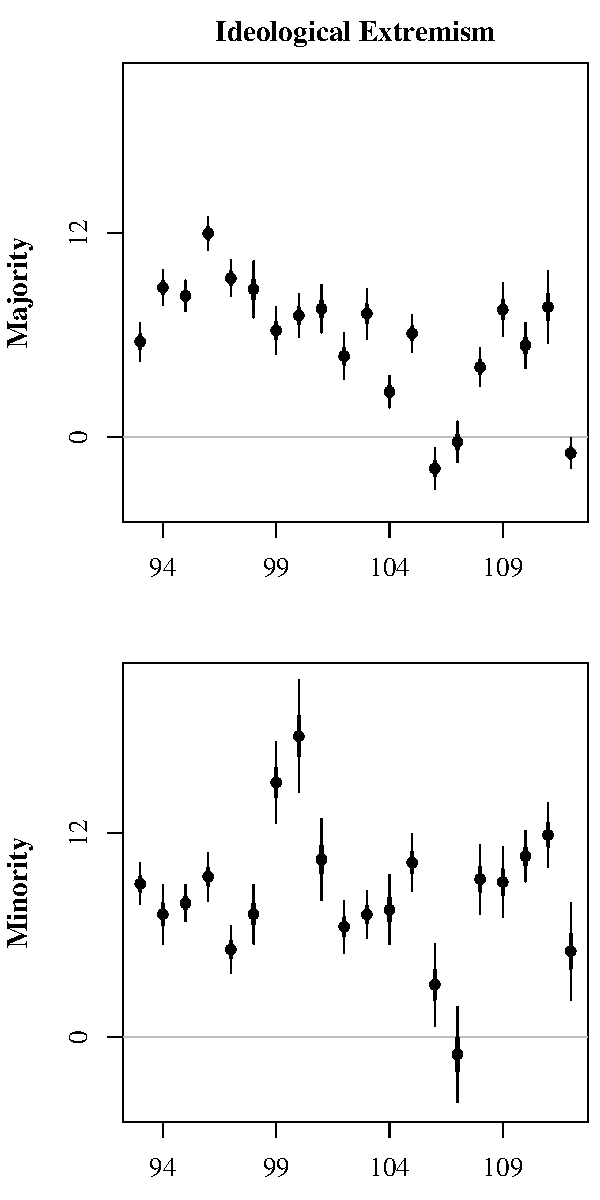
\includegraphics[width = 10cm]{C:/Users/Ethan/Documents/GitHub/partycalls/plots/who-heeds-figure2-replication_lm.pdf}
\end{figure}

\begin{figure}[H]
	\centering
	\caption{Senate Ideological Extremism Coefficient Plot}
	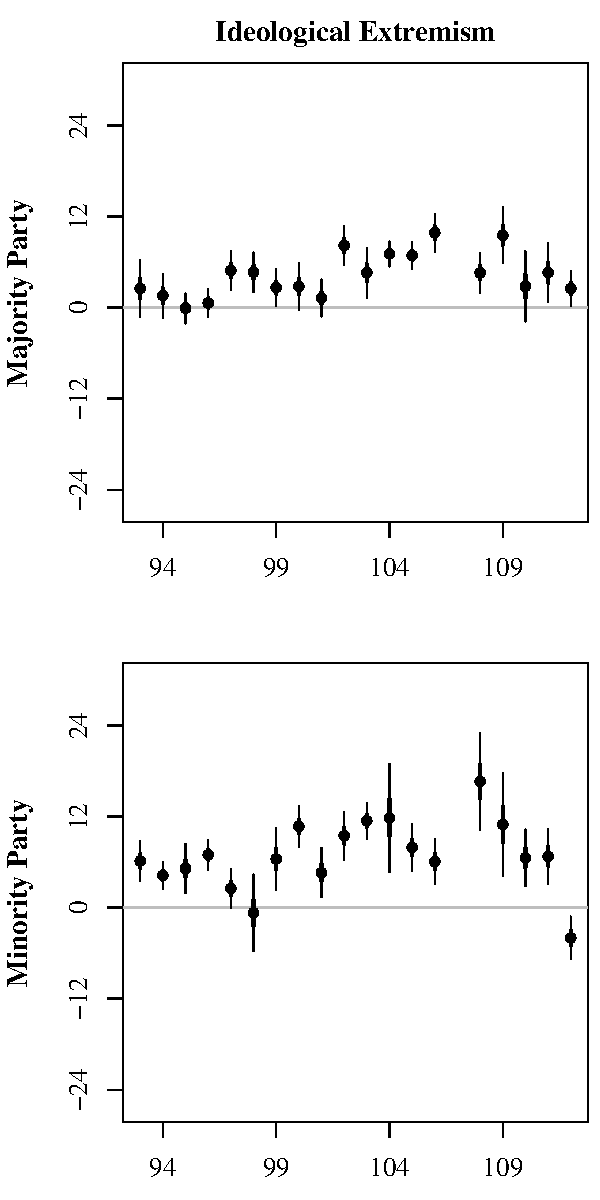
\includegraphics[width = 10cm]{C:/Users/Ethan/Documents/GitHub/partycalls/plots/senate-figure2-lm.pdf}
\end{figure}





















































\end{document}